%
% This is Chapter 6 file (chap6.tex)
%
\chapter{Temperature Enhancement Along Intermittent Structures}\label{chap:chap6}

    \section{Overview} \label{sec:ovrvw6}

        The solar wind proton temperature at 1\,au has been found to be correlated with small-scale
        intermittent magnetic structures, i.e., regions with enhanced temperature are associated
        with coherent structures such as current sheets. Using Parker Solar Probe data from the
        first encounter, we study this association using measurements of radial proton temperature,
        employing the Partial Variance of Increments (PVI)\index{PVI} technique to identify intermittent
        magnetic structures. We observe that the probability density functions of high-PVI events
        have higher median temperatures than those with lower PVI, The regions in space where PVI
        peaks were also locations that had enhanced temperatures when compared with similar regions
        suggesting a heating mechanism in the young solar wind that is associated with intermittency
        developed by a nonlinear turbulent cascade in the immediate vicinity. We also look into
        magnetosheath ion temperature using MMS and report on the findings.\footnote{Part of this
        study was published in \citet{Qudsi2020}.}

    \section{Introduction} \label{sec:intr6}

        As discussed in \Cref{sec:plas2}, solar wind is a stream of charged and highly magnetized
        plasma streaming at supersonic speed originating from the Sun. Solar wind is primarily
        composed of ionized hydrogen \citep{Marsch1982a, Kasper2012} with varying amount of helium
        nucleus \citep{Maruc2012} and minor heavier ions.

        Despite decades of observation, the exact process that originally heats and accelerates
        solar wind plasma remain unknown, but several candidates have been proposed. Turbulence
        cascade transfers energy from large to small scales (see \Cref{sec:inter3b} for more
        details), which can ultimately lead to dissipation and heating \citep{Velli1989, Velli1993,
        Matthaeus1999, Dmitruk2002, Cranmer2005, Cranmer2007, Cranmer2012, Cranmer2014, Verdini2007,
        Verdini2009, Verdini2009a, Chandran2009, Perez2013, Lionello2014}. Current sheets, generated
        by cascading vortices, can also lead to localized heating \citep{Parashar2009, Osman2011,
        Osman2012, Osman2012a, Gingell2015}. Wave particle interactions --- including, e.g.,
        microinstabilities, Landau damping, and ion-cyclotron resonance --- can likewise result in
        significant changes to the particles' phase-space distribution \citep{Gary1993,
        Sahraoui2010, Klein2015}. Though there are several linear and non-linear mechanisms which
        heats the space plasma, here we focused on one such mechanism, coherent structures: features
        in the plasma that are persistent through time, concentrated in space, or both
        \citep{Greco2018}. As discussed in \Cref{sec:intmt} such structures can be produced by
        turbulent cascade \citep{Osman2012a} and are also associated with current sheets
        \citep{Yordanova2016}. \citet{Osman2011, Osman2012a} analyzed in-situ observations and of
        near-Earth solar wind and found clear indications that coherent structures correlate with
        local enhancements in temperature.

        So far most of the studies have been done using either numerical simulation data or solar
        wind data at 1\,au. However, plasma conditions are a lot different at 1\,au from those very
        close to the Sun, say 0.2\,au. Magnetic field near 0.2\,au is $\sim$\,70\,nT compared to
        $\sim$\,5\,nT at 1\,au. Plasma at 0.2\,au is also much denser and hotter ($\sim$\,200\,
        /$\mathrm{cm^{-3}}$ and $\sim\,10^6$\,K compared to $\sim$\,5\,/$\mathrm{cm^{-3}}$ and
        $\sim\,10^4$\,K respectively) \citep{Kasper2019}. And even though solar wind is mostly
        collisionless, plasma at 1\,au has gone through more processing compared to the young solar
        wind \cite[\S3.3 \& references therein]{Verscharen2019}. The recently launched Parker Solar
        Probe (PSP) provides an unprecedented opportunity to study the nascent solar wind in great
        detail.

        In this study, we revisit the techniques of \citet{Osman2011, Osman2012a}, and, by applying
        them to observations from
        \discolorlinks{\href{https://www.nasa.gov/content/goddard/parker-solar-probe}{Parker Solar
        Probe}} (PSP), explore the relationship between plasma structures and heating in nascent
        solar wind plasma. We also look into the heating of terrestrial magnetosheath plasma using
        data from MMS. \Cref{sec:bgnd6} provides the background on such structures and introduces
        the reader to the physics of technique employed in data analysis which is described in
        \Cref{sec:data6}. In \Cref{sec:diss6} we present the results and discuss its implication.
        \Cref{sec:conc6} summarizes the results along with a conclusion and potential future works.

    \section{Background} \label{sec:bgnd6}

        Some recent studies, both observational and numerical, have shown that intermittent
        structures are correlated with the regions of enhanced temperature in the plasma
        \citep{Osman2012, Osman2011, Greco2012} and understanding the mechanisms by which the
        turbulence heats the plasma may also help solve the coronal heating problem
        \citep{Osman2012a}. This is a particularly attractive scenario especially given the ubiquity
        of the localized structures. Study performed on data from PIC simulation by \citet{Wu2013}
        shows that the correlation between enhanced temperature and coherent structures exists for
        sub ion inertial length ($d_{\rm i}$). Further evidence of this is provided by
        \citet{TenBarge2013} for Gyrokinetic simulation, \citet{Parashar2009, Wan2012,
        Karimabadi2013, Wan2015} for PIC and \citet{Servidio2012, Servidio2015} for Vlasov
        simulations respectively. Work done by \citet{Chasapis2015} and \citet{Yordanova2016} on
        from Cluster and MMS data show similar results from observation vantage point.

        In this study, we investigate these discontinuities in the magnetic field and explore their
        association with local enhancements in ion temperature. As discussed in \Cref{sec:intmt} we
        use PVI (see \Cref{eq:pvi} for the expression of PVI) to identify the discontinuities.
        Although these structures constitute only a small fraction of total data set their
        contribution to the total internal energy per unit volume is high. This emphasizes the
        importance of using the PVI technique for such studies. We also note that an analogous
        examination of the association of PVI events with energetic particles was carried out at
        1\,au, \citep{Tessein2016}.

    \section{Data Selection and Methodology} \label{sec:data6}

        We analyzed data from PSP's first encounter with the Sun (October 31 to November 11, 2018).
        The FIELDS fluxgate magnetometers provided measurements of the local magnetic field at a
        rate of 64\,samples/NYseconds. Radial proton temperature/thermal speed data was obtained
        from the Solar Probe Cup (SPC), part of the Solar Wind Electron, Alpha and Proton suite
        \citep{Kasper2016} (See \Cref{sec:psp} for a more detailed discussion of PSP, SPC, FIELDS
        and the dataset used in this study). The average speed of solar wind during the first
        encounter was around 350\,km/s for the most part and crossed 500\,km/s only on the last day
        of the encounter. Thus, using Taylor’s Hypothesis, 1\,NYs corresponds to a length scale of
        300\,km.

        For the calculation of PVI according to \Cref{eq:pvi}, we used 64\,NYHz data, with a lag of
        1\,NYs, which is the native cadence of SPC \citep{Kasper2016}. The ensemble averaging was
        done over 8\,hours, which is several times the estimated correlation time. In this study we
        used the correlation time computed in \citet{Parashar2020}. However there are few subtleties
        associated with this calculation, and \citet{Smith2001, Isaacs2015, KrishnaJagarlamudi2019,
        Bandyopadhyay2020} offer more insights and discussion on this topic along with potential
        issues in such determination. We also carried out the analysis for various different
        averaging times (from 1 to 12\,hours) and different lags (from 1 to 100\,seconds) and it was
        observed to have minimal affect on the outcome. \Cref{fig:pvi_comp_psp} plots the relative
        changes in PVI for $6^{th}$ of November, 2018 for these different inputs, and shows that the
        value of computed PVI barely changes for different lags and averaging times, thereby
        reaffirming the robustness of this method. Though changing the lag or averaging times or
        both slightly changes the overall value of PVI, they remain highly correlated with respect
        to each other over the entire interval. PVI time series was then resampled to ion cadence of
        1\,NYHz in the way such that for each interval of 1\,NYs, the maximum value of PVI in that
        interval was chosen.

        \begin{sidewaysfigure}
            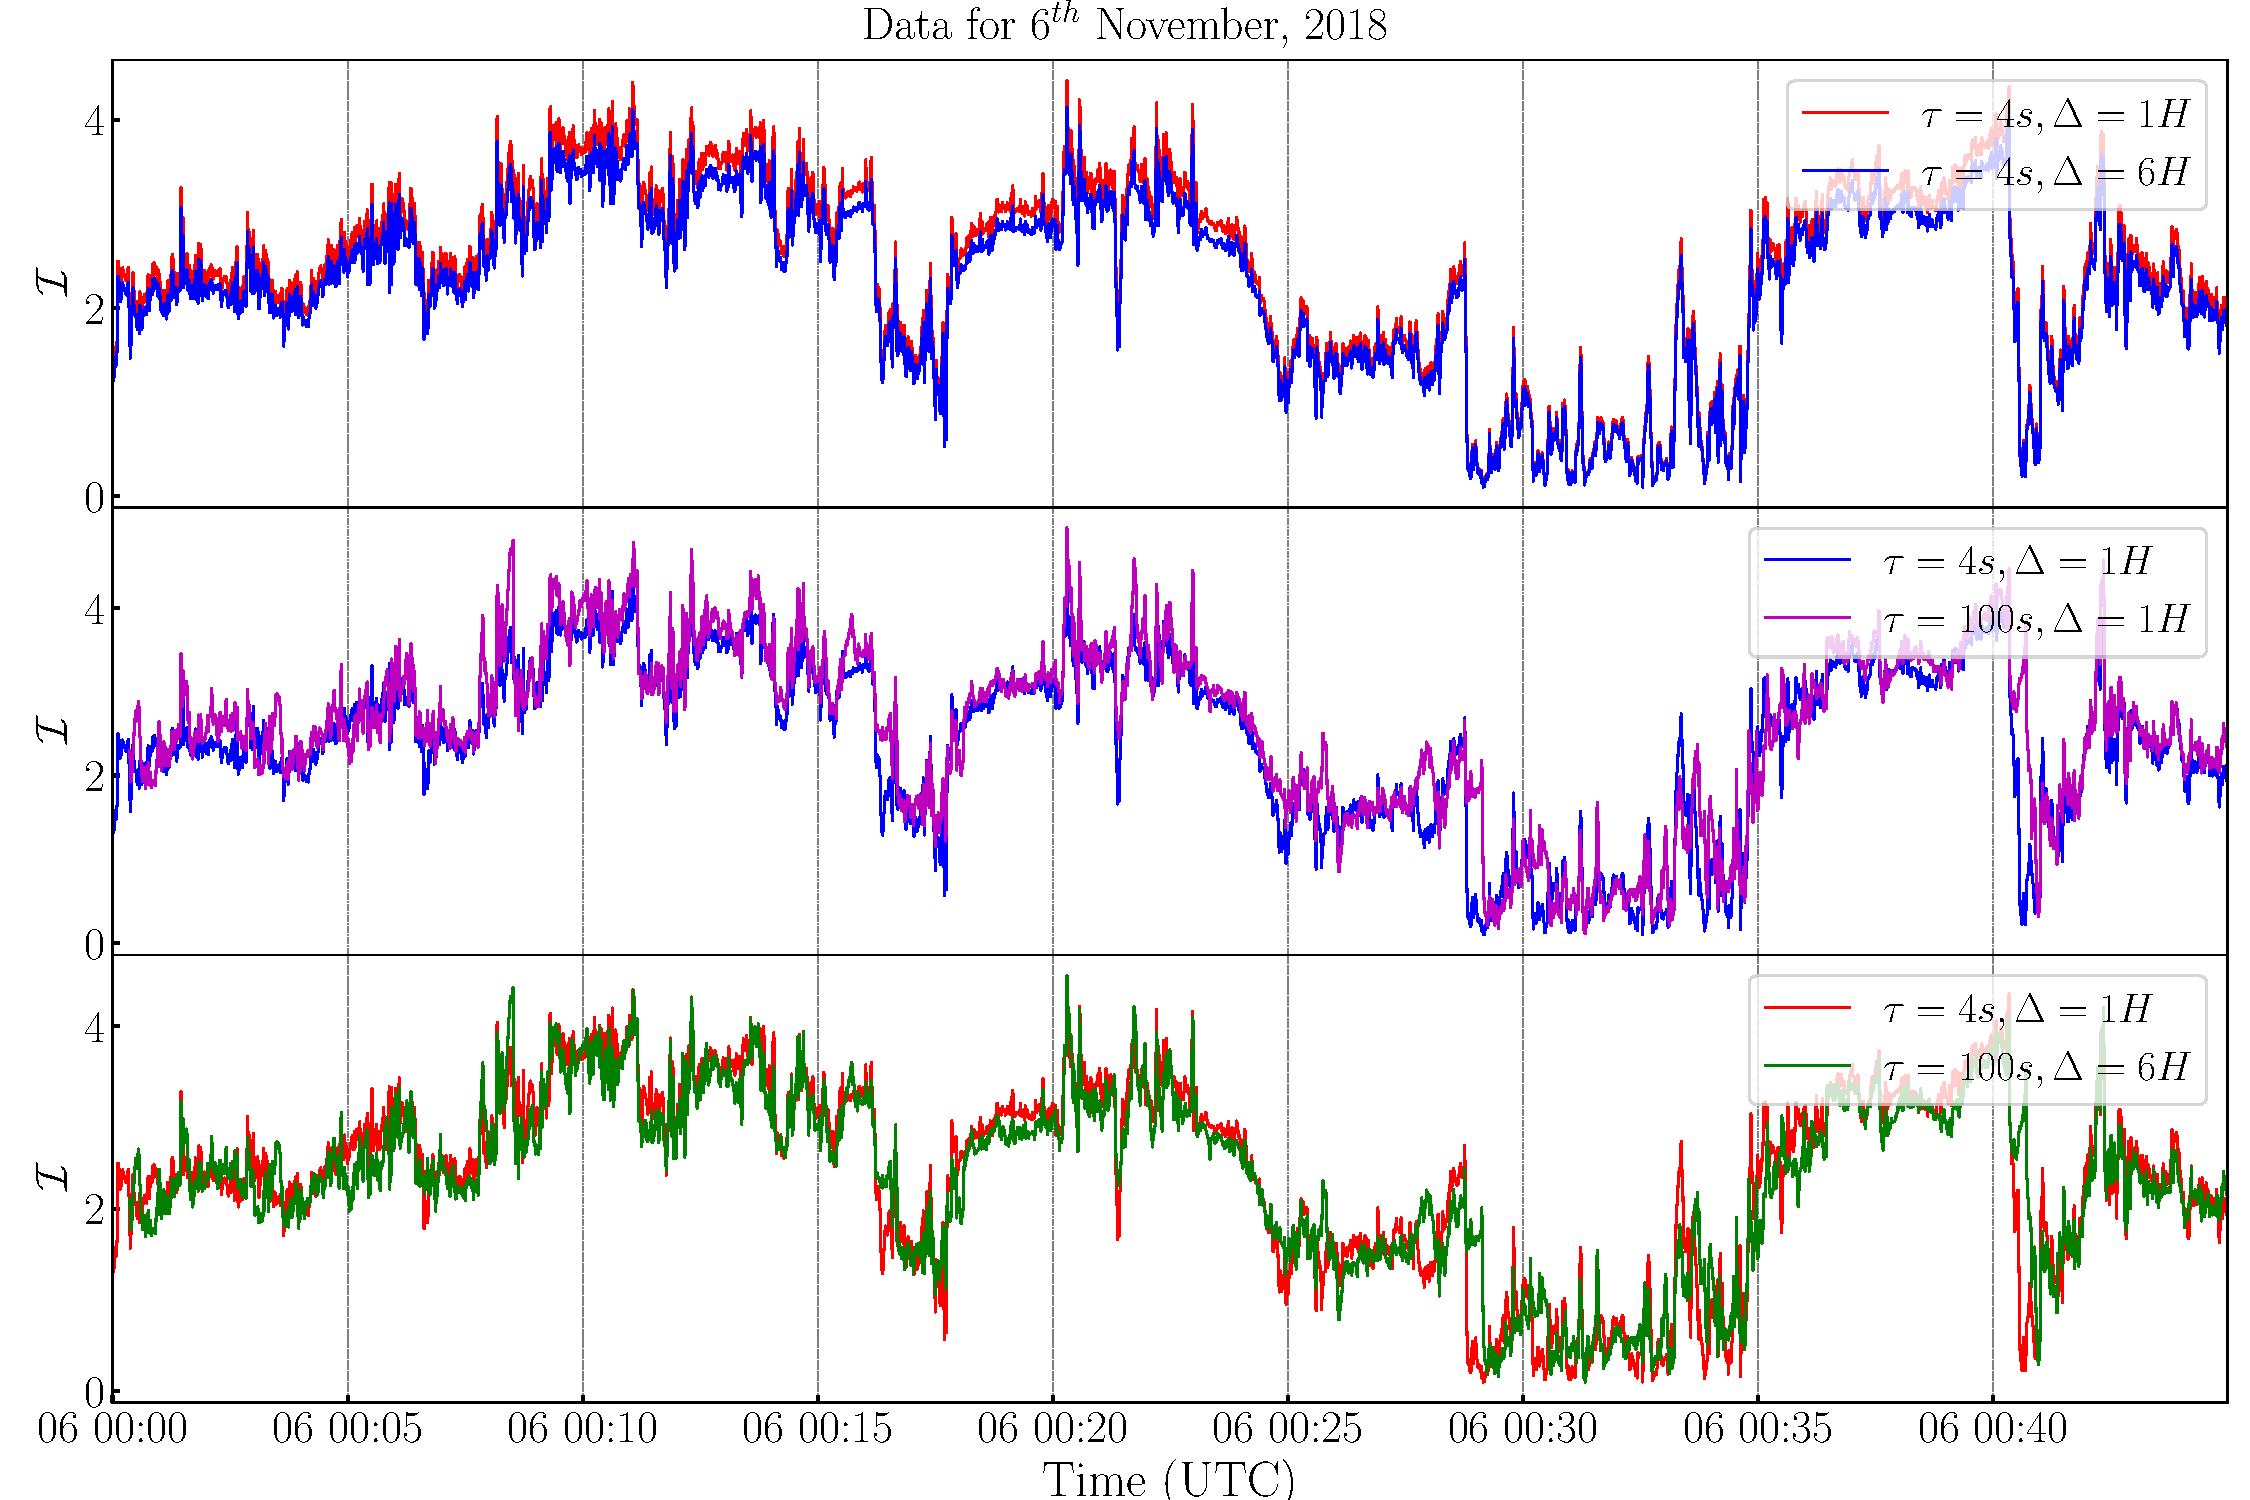
\includegraphics[width=1.\textwidth]{figures/chap6/pvi_comp_psp.pdf}
            \caption[$\mathcal{I}$ comparisons for different $\tau$]{Comparison of PVI computed for
            PSP for various different set of lag and averaging time. Though changing the lag or
            averaging times or both slightly changes the overall value of PVI, they remain highly
            correlated with respect to each other over time.}
            \label{fig:pvi_comp_psp}
        \end{sidewaysfigure}

        In this study we focused on the second half of the encounter, immediately after PSP was at
        its perihelion. The second half of the encounter has very different properties compared to
        the first half. A greater number of energetic particles were observed \citep{McComas2019},
        the solar wind speed was comparatively higher \citep{Kasper2019}, and there were many more
        switchbacks or polarity reversal of magnetic fields \citep{Bale2019}.
        \citet{Bandyopadhyay2020} observed enhanced local energy transfer, which points towards a
        more turbulent period in general, and thus a suitable environment for PVI study.

        For MMS analysis, we used the same data set as reported in \Cref{sec:sco5,sec:mms}.

    \section{Results} \label{sec:diss6}

        \begin{figure}
            \begin{center}
                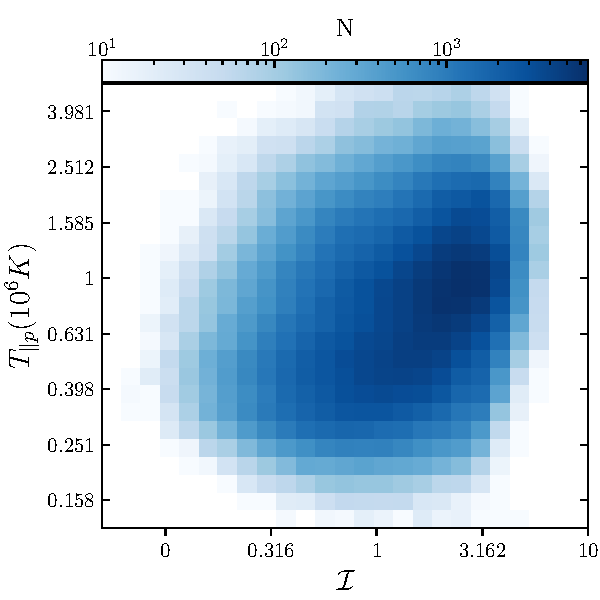
\includegraphics[width=1.\textwidth]{figures/chap6/PVIvsT_hist_masked_lin_mag_psp_par.pdf}
                \caption[Joint histogram of $T_{\parallel p}$ and $\mathcal{I}$]{Joint histogram of
                radial proton-temperature and PVI for the second half of first encounter on a
                log-log scale. There is an upward trend between PVI and temperature as the deep blue
                region in the plot tilts upwards showing an increase of temperature as PVI
                increases. \textit{Figure reproduced from \citet{Qudsi2020} with the permission of
                \href{https://publishing.aip.org/}{AIP Publishing}} (see
                \Cref{apdx:D}).}
                \label{fig:pvi_hst_psp}
            \end{center}
        \end{figure}

        \begin{figure}
            \begin{center}
                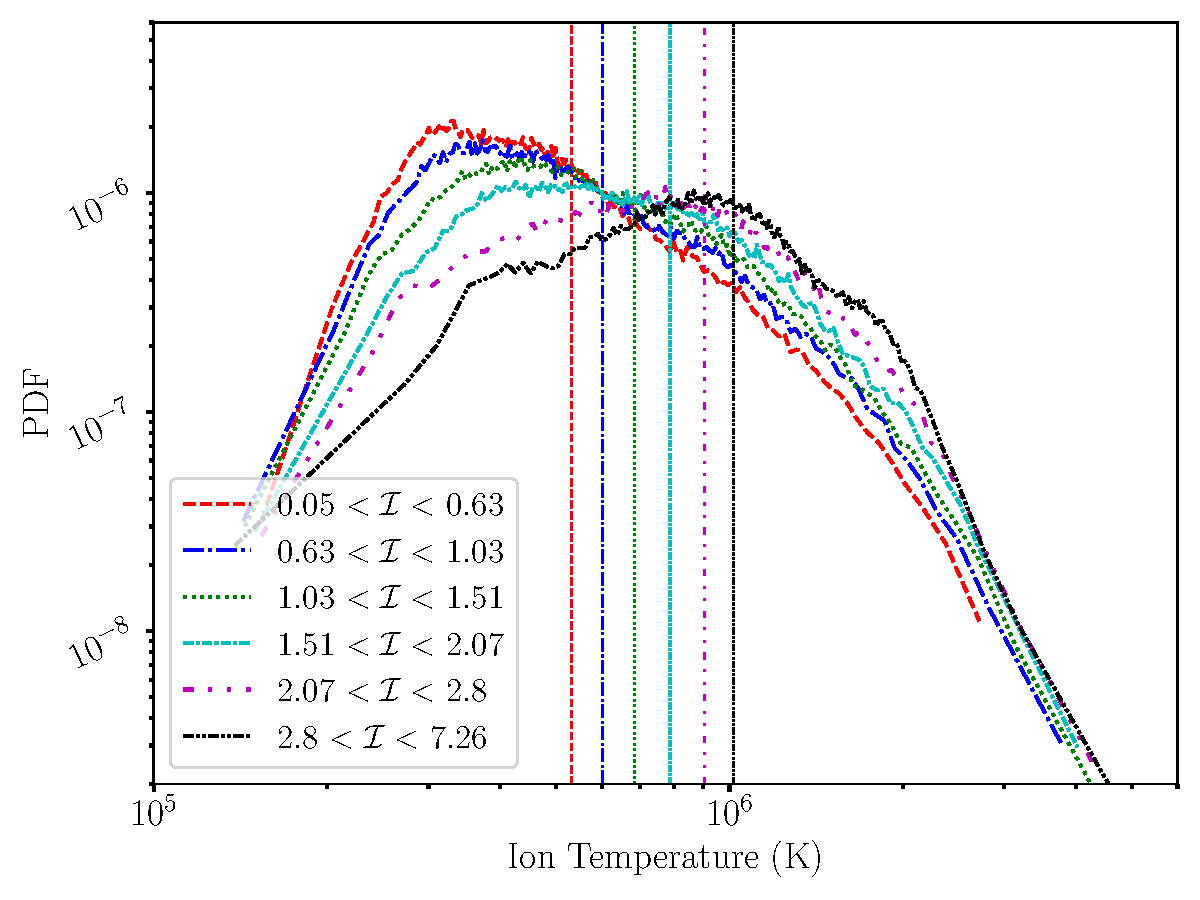
\includegraphics[width=1.\textwidth]{figures/chap6/T_pdf_pvi_psp.pdf}
                \caption[PDF of $T_{\rm \parallel p}$ for various $\mathcal{I}$ for \texttt{psp}
                dataset]{PDFs for the radial proton-temperature for the second half of first
                encounter. Each PDF corresponds to a different PVI range such that each PVI bin has
                equal number of data points. The probability density increases with increase in
                temperature for high PVI events and peaks at comparatively higher value of
                temperature, whereas it decreases for low PVI PDF. Vertical lines show the median
                temperature for each of the PDF plot. \textit{Figure reproduced from
                \citet{Qudsi2020} with the permission of \href{https://publishing.aip.org/}{AIP 
                Publishing}} (see \Cref{apdx:D}).}
                \label{fig:pvi_pdf_psp}
            \end{center}
        \end{figure}

        %\begin{figure} \begin{center}
        %    \includegraphics[width=1.\textwidth]{figures/chap6/%PVIvsT_hist_masked_lin_mag_mms_total.pdf}
        %    \caption{Joint histogram of total proton-temperature and PVI for the 40 minutes burst
        %    observation from MMS. Unlike the PSP case there doesn't seem to be a positive trend
        %    between temperature and PVI.} \label{fig:pvi_hst_mms} \end{center} \end{figure}

        \begin{figure}
            \begin{center}
                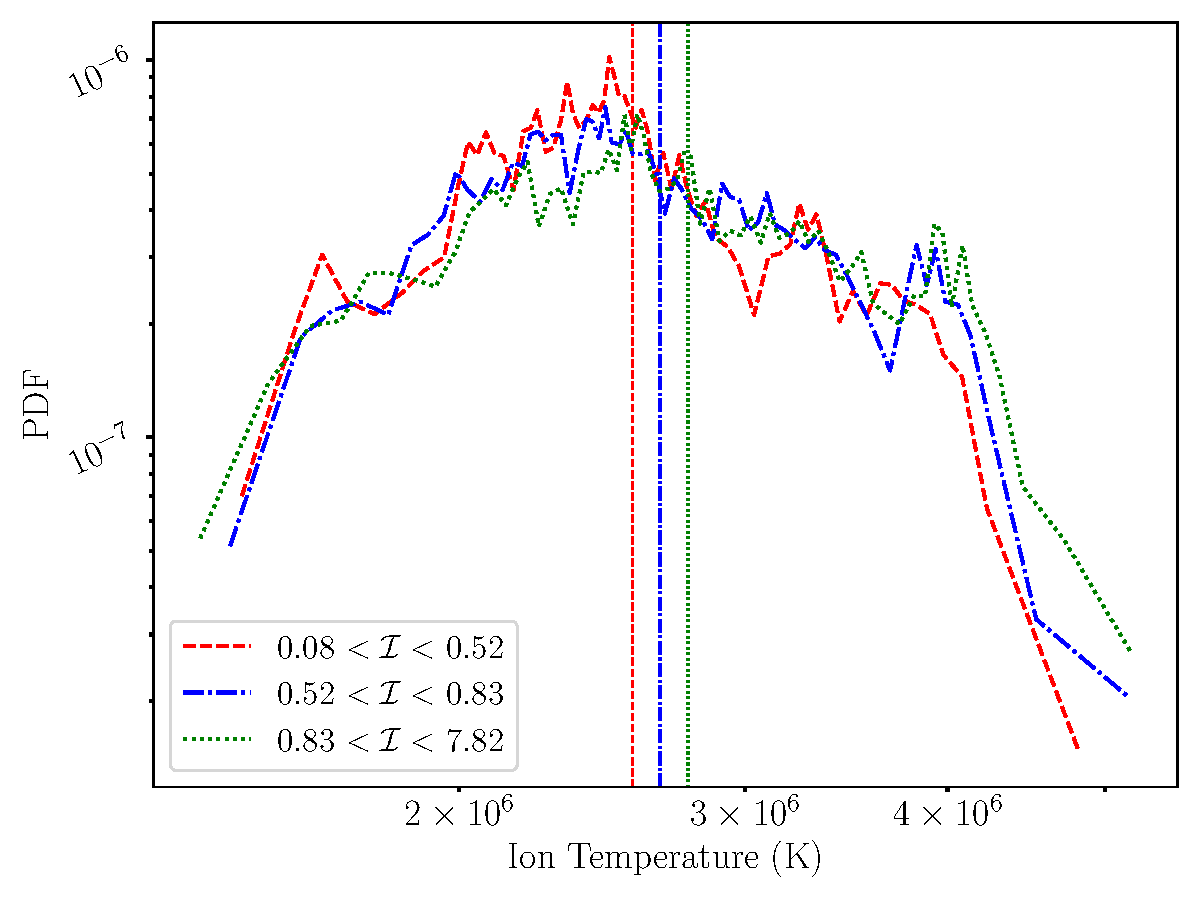
\includegraphics[width=1.\textwidth]{figures/chap6/T_pdf_pvi_mms_20171226_4.pdf}
                \caption[PDF of $T_{\rm \parallel p}$ for various $\mathcal{I}$ for \texttt{mms}
                dataset]{PDFs for the total proton-temperature for 40 minutes burst observation from
                MMS. Each PDF corresponds to a different PVI range such that each PVI bin has equal
                number of data points. The probability density increases with increase in
                temperature for high PVI whereas it decreases for low PVI PDF. Vertical lines show
                the median temperature for each of the PDF plot.}
                \label{fig:pvi_pdf_mms}
            \end{center}
        \end{figure}

        \Cref{fig:pvi_hst_psp} shows the joint histogram of radial proton-temperature and PVI for
        the first encounter of PSP. Increasing PVI color contours have an upwards trend, as we see
        temperature distribution showing a positive slope with increase in value of PVI. The
        positive correlation between temperature and PVI suggest some kind of heating in the regions
        with high PVI. We then conditionally sampled radial proton temperature. Conditionally
        sampled means that we arrange the data by increasing value of PVI and then divide all the
        data points in 6 bins such that each bin has equal number of points. We then calculate the
        temperature distribution within each bin which is shown in \Cref{fig:pvi_pdf_psp}.

        As PVI increases, the probability density increases for the higher temperature and decreases
        for the lower temperature which is opposite of what we see at the low temperatures where
        probability density is highest for the lowest PVI. Median temperature, shown by vertical
        lines in \Cref{fig:pvi_pdf_psp}, for each of the distribution increases implying presence of
        stronger and stronger heating as we go to higher and more extreme values of PVI. For PVI $<$
        1, median value of the temperature is $5.32 \times 10^5$\,K whereas for PVI $>$ 6, the
        median temperature increases to $1.01 \times 10^6$\,K. \citet{Osman2011} observed similar
        increase in average temperature in their study of solar wind at 1\,au. This is consistent
        with heating occurring in the regions with small scale coherent structure in MHD turbulence.

        Though distribution of total proton temperature from magnetosheath shows similar trend in
        the median temperature of each bin as seen in \Cref{fig:pvi_pdf_psp}, the enhancement in
        temperature is comparatively smaller. The median temperature corresponding to three bins
        shown in \Cref{fig:pvi_pdf_psp} are $2.56 \times 10^6$\,K, $2.66 \times 10^6$\,K and $2.77
        \times 10^6$\,K, which is barely an increment. However, this is reflective of two features
        of magnetosheath temperature and PVI compared to that of nascent solar wind. The radial
        temperature of solar wind varies over more than an order of magnitude whereas for
        magnetosheath it is less than half an order. Also, comparatively, solar wind has much higher
        values of PVI than that of magnetosheath, mean value of $1.69$ versus $0.78$. There are
        other factors to be considered as well. Short interval of observation which results in
        smaller amount of data could be another contributing factor. Also, in the case that
        fluctuation event lasts longer than the interval length, we won't detect any enhancement in
        the observed temperature. Though we did not see a conclusive evidence of temperature
        enhancement for ions, it is worth noting that \citet{Chasapis2018} did observe it for
        electrons. A comparative statistical study of PVI for datasets of different length of
        observation time will can help in quantifying how prominent is the effect of duration of
        observations on the value of computed PVI.

        In order to further demonstrate the relationship between PVI and enhanced temperature for
        PSP, we looked at the temperature at the point of high PVI event and its immediate
        surrounding in space using the methodology described by \citet{Osman2012a}. We compute the
        mean value of temperature at the point of the PVI event and for points near the PVI events
        separated from it by up to one correlation length. Formally, these averages may be expressed
        as:
        \begin{align}
            \widetilde{T}_{\rm p}( \delta t, \theta_{\rm 1}, \theta_{\rm 2}) = \langle T_{\rm p}(t_{\mathcal{I}}+\delta t)| \theta_{\rm 1} \leq \mathcal{I}(t_\mathcal{I}) < \theta_{\rm 2} \rangle \label{eq:tts}
        \end{align}
        where $\widetilde{T}_{\rm p}$ is the conditionally averaged temperature for all the events,
        $\delta t$ is the time difference relative to the position of PVI events, $t_\mathcal{I}$ is
        the time of PVI events between the threshold $\theta_{\rm 1}$ and $\theta_{\rm 2}$. In
        \Cref{eq:tts}, for a given threshold of PVI, we record the temperature at each point where
        PVI satisfies the expression $\theta_{\rm 1} \leq \mathcal{I}(t_\mathcal{I}) < \theta_{\rm
        2}$. We then record the temperature around that point, moving up to 1 correlation length
        away from the point of PVI event. Once we have the temperature at all such points, we take
        the average of all temperatures which were at same distance from the event.

        \begin{figure}
            \begin{center}
                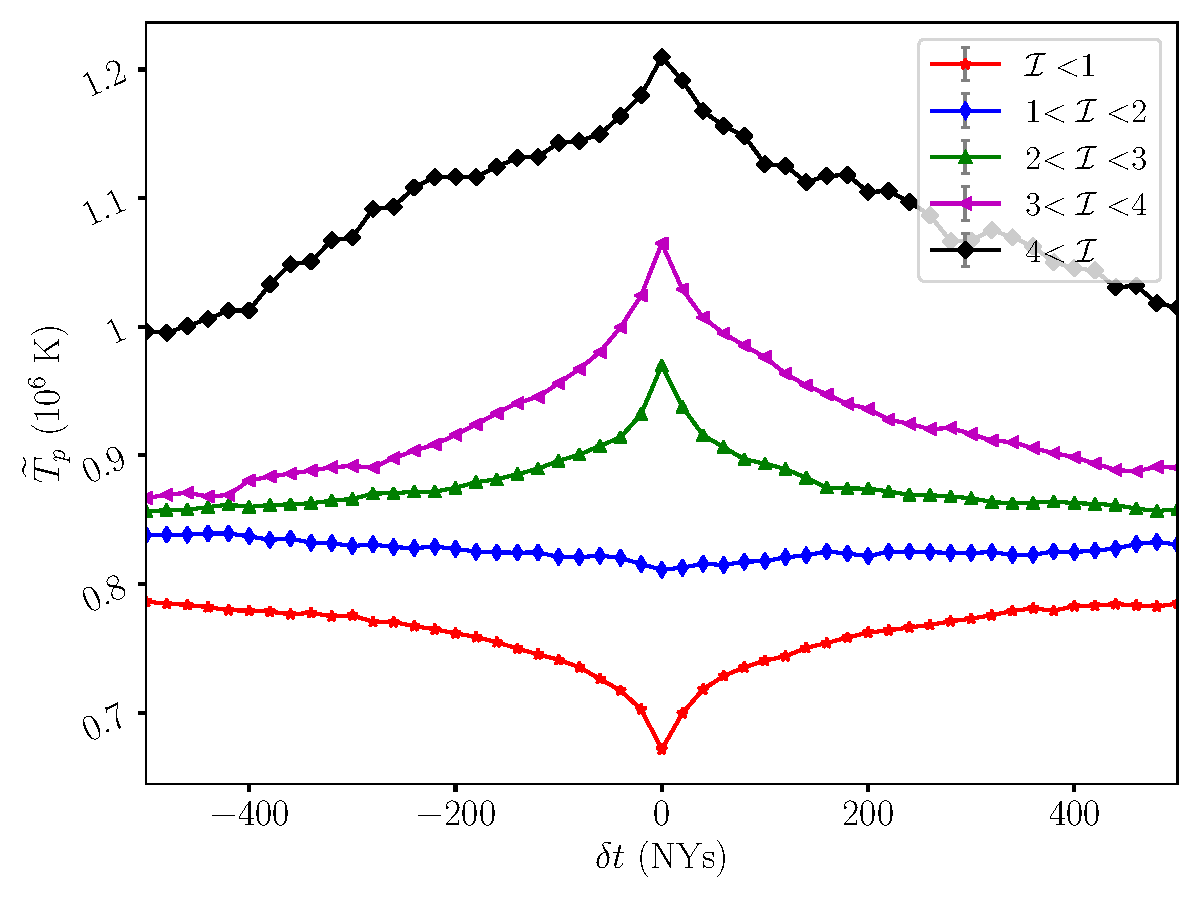
\includegraphics[width=1.\textwidth]{figures/chap6/tem_pvi_lag_psp.pdf}
                \caption[Conditionally averaged $T_{\rm \parallel p}$ from a $\mathcal{I}$
                event]{Figure shows conditional average temperature for different PVI thresholds at
                the point of a PVI event. $\widetilde{T}_{\rm p}$ peaks at the instant of PVI event
                and continues to have elevated temperature in its vicinity within the correlation
                time scale. Red curve, corresponding to lowest PVI shows a dip suggesting no heating
                when the magnetic field is very smooth. The error bars are smaller than the symbols
                and thus not easily visible in the figure. \textit{Figure reproduced from
                \citet{Qudsi2020} with the permission of \href{https://publishing.aip.org/}{AIP
                Publishing}} (see \Cref{apdx:D}).}
                \label{fig:tem_pvi_lag}
            \end{center}
        \end{figure}

        \Cref{fig:tem_pvi_lag} shows the plot of $\widetilde{T}_{\rm p}$ for various thresholds for
        the second half of the encounter. Not only do we observe enhanced temperature at the point
        of high PVI events, suggesting localized heating at those points, we also see that
        $\widetilde{T}_{\rm p}$ for a higher PVI event is consistently higher than nearby points
        separated by up to a correlation length. This implies that the points nearby an identified
        PVI event have an elevated average temperature, continuously approaching the elevated
        average temperature found at the PVI event itself. Some of this effect may be due to
        clustering of PVI events (see \citet{Chhiber2020}). Another point worth noting in
        \Cref{fig:tem_pvi_lag} is the valley in the temperature profile for small PVI. This is the
        region where background magnetic field is smooth and it appears that in such regions, the
        temperature is lower than the temperature of plasma in its immediate surrounding, which is
        concurrent with the fact that in those places there is no turbulence heating.
        \citet{Osman2012a} found similar result in their study at 1\,au. However, in our study we
        find a significant dip compared to the dip reported in \citet{Osman2012a}, $\sim 10^5$\,K
        compared to $\sim 2\times 10^3$\,K.

    \section{Discussions} \label{sec:conc6}

        In this study, we used in-situ observations from PSP's first encounter with the Sun and the
        magnetosheath data from MMS to explore the association of proton heating with coherent
        magnetic structures in space plasmas. We identified enhancements of PVI \citep{Greco2008} as
        indicative of the presence of such a structure \citep{Osman2011, Osman2012a}. We observed
        that the joint histogram of PVI and proton radial temperature, for solar wind, shows
        positive trend as shown in \Cref{fig:pvi_hst_psp}. We also observed that the PDF of data, as
        shown in \Cref{fig:pvi_pdf_psp,fig:pvi_pdf_mms}, with higher PVI has higher median
        temperature compared to those with lower PVI for both solar wind and terrestrial
        magnetosheath. These observations strongly supports the theory that the solar wind in those
        regions are heated by coherent structures which are generated by plasma turbulence. Though
        owing to certain characteristics of magnetosheath data, a more in-depth analysis is required
        to draw any final conclusion.

        The present results demonstrate both the shifting of the PDF of temperature towards higher
        values with increasing PVI condition, (in \Cref{fig:pvi_pdf_psp}) and the spatial/temporal
        localization of the temperature enhancement near PVI events (in \Cref{fig:tem_pvi_lag}).
        Both of these are fully consistent with findings in the two papers that examine these
        effects (\citet{Osman2011, Osman2012}, respectively). It is interesting that these effects
        are present clearly in the PSP first orbit where turbulence is presumably younger and
        possibly less well developed than it is at 1\,au. It is possible that the temperature
        differential between low and high PVI is somewhat less in the PSP data than in the ACE data
        at 1\,au \citep{Osman2011}, but additional samples by PSP will be needed to draw any firm
        conclusion of this type.

        In order to further demonstrate this association we looked at the conditionally average
        temperatures at the point of a high PVI event and in its immediate surrounding up to
        1\,correlation length. We observed that not only the point of event has the highest
        temperature, its vicinity shows enhanced temperature compared to lower PVI events. The local
        maxima of these temperature profiles are most prominent for higher PVI events suggesting
        stronger heating. The plateau region of each thresholds are distinct, and for higher
        threshold they maintain a high value suggesting clustering of PVI events around a large
        discontinuity. For very smooth magnetic field we see a dip in the average temperature at
        that point. \citet{Osman2012a} found similar behavior in their study of solar wind at 1\,au,
        though neither the heating nor the dip in temperature for small PVI that they reported in
        their study was as high as what we observed in our study. This suggests that either coherent
        structures are more efficient in heating the plasma near the Sun compared to 1\,au or we
        have a lot more such structures as we move closer to the Sun. Since these coherent
        structures are generated by plasma turbulence, these observations suggest that non-linear
        turbulence cascade play a crucial role in heating the nascent solar wind. Given the
        ubiquitous nature of such structures, this process can help explain the coronal heating or
        be at least a part of the explanation.

        A significant limitation of this study was unavailability of temperature-anisotropy data.
        The temperature measures we used were not the scalar temperature but rather the radial
        temperature, for which reason we limited our observations to period of nearly-radial
        magnetic field (see \Cref{sec:data6,sec:psp}). Once reliable ion temperature-anisotropy data
        are available, the present study could be revisited to explore both scalar and anisotropic
        heating. Theoretical studies have found that turbulent cascade can generate strong
        temperature anisotropy near coherent structures \citep{Parashar2016}.

        A careful inspection of \Cref{fig:tem_pvi_lag} reveals a very slight asymmetry in the shape
        of the temperature profile right before and after the PVI event. The phenomenon was also
        noted in 1\,au solar wind by \citep{Osman2012a}. The cause and significance of this
        asymmetry remain unclear, but it may it suggests a connection between local heating and
        large-scale processes such as heat flux.